\documentclass[UTF8,12pt]{article}
\usepackage{ctex}
\usepackage{indentfirst}
\usepackage{color}
\usepackage{hyperref}
\usepackage{graphicx}
\usepackage{subfigure}
\usepackage{pdfpages}
\usepackage{listings}
\hypersetup{
    hidelinks,
	colorlinks=true,
	allcolors=black,
	pdfstartview=Fit,
	breaklinks=true
}

\definecolor{dkgreen}{rgb}{0,0.6,0}
\definecolor{gray}{rgb}{0.5,0.5,0.5}
\definecolor{mauve}{rgb}{0.58,0,0.82}

\lstset{ %
  language=Octave,                % the language of the code
  basicstyle=\footnotesize,           % the size of the fonts that are used for the code
  numbers=left,                   % where to put the line-numbers
  numberstyle=\tiny\color{gray},  % the style that is used for the line-numbers
  stepnumber=2,                   % the step between two line-numbers. If it's 1, each line 
                                  % will be numbered
  numbersep=5pt,                  % how far the line-numbers are from the code
  backgroundcolor=\color{white},      % choose the background color. You must add \usepackage{color}
  showspaces=false,               % show spaces adding particular underscores
  showstringspaces=false,         % underline spaces within strings
  showtabs=false,                 % show tabs within strings adding particular underscores
  frame=single,                   % adds a frame around the code
  rulecolor=\color{black},        % if not set, the frame-color may be changed on line-breaks within not-black text (e.g. commens (green here))
  tabsize=2,                      % sets default tabsize to 2 spaces
  captionpos=b,                   % sets the caption-position to bottom
  breaklines=true,                % sets automatic line breaking
  breakatwhitespace=false,        % sets if automatic breaks should only happen at whitespace
  title=\lstname,                   % show the filename of files included with \lstinputlisting;
                                  % also try caption instead of title
  keywordstyle=\color{blue},          % keyword style
  commentstyle=\color{dkgreen},       % comment style
  stringstyle=\color{mauve},         % string literal style
  escapeinside={\%*}{*)},            % if you want to add LaTeX within your code
  morekeywords={*,...}               % if you want to add more keywords to the set
}


\setlength{\parindent}{2em}

\begin{document}



\begin{center}
    \tableofcontents
\end{center}
\newpage

\section{实验目的与要求}
\subsection{实验目的}
首先学习面向TCP连接的套接字编程基础知识:如何创建套接字,将其绑定到特定的地址和端口,以及发送和接收数据包。其次还将学习 HTTP 协议格式的相关知识。在此基础上,本实验开发一个简单的 Web 服务器,它仅能处理一个HTTP连接请求。
\subsection{实验要求}
Web 服务器的基本功能是接受并解析客户端的 HTTP 请求,然后从服务器的文件系统获取所请求的文件,生成一个由头部和响应文件内容所构成成的 HTTP 响应消息,并将该响应消息发送给客户端。如果请求的文件不存在于服务器中,则服务器应该向客户端发送“404 Not Found”差错报文。 具体的过程和步骤分为:
\begin{enumerate}
    \item 当一个客户(浏览器)连接时,创建一个连接套接字;
    \item 从这个连接套接字接收 HTTP 请求; 
    \item 解释该请求以确定所请求的特定文件; 
    \item 从服务器的文件系统获得请求的文件;
    \item 创建一个由请求的文件组成的 HTTP 响应报文,报文前面有首部行; 
    \item 经 TCP 连接向请求浏览器发送响应;
    \item 如果浏览器请求一个在该服务器中不存在的文件,服务器应当返回一个“404 Not Found”差错报文。
\end{enumerate}

\section{实验原理与实验内容}
\subsection{实验原理}
\subsubsection{Socket编程接口}
要实现 Web 服务器,需使用套接字 Socket编程接口来使用操作系统提供的网络通信功能。 Socket 是应用层与 TCP$/$IP 协议族通信的中间软件抽象层,是一组编程接口。它把复杂的 TCP$/$IP 协议族隐藏在 Socket 接口后面,对用户来说,一组简单的接口就是全部,让 Socket 去组织数据,以符合指定的协议。使用 Socket 后,无需深入理解 TCP$/$UDP 协议细节(因为Socket 已经为我们封装好了),只需要遵循 Socket 的规定去编程,写出的程序自然就是遵循 TCP$/$UDP 标准的。Socket 的地位如下图所示:
\begin{figure}[htbp]
    \centering
    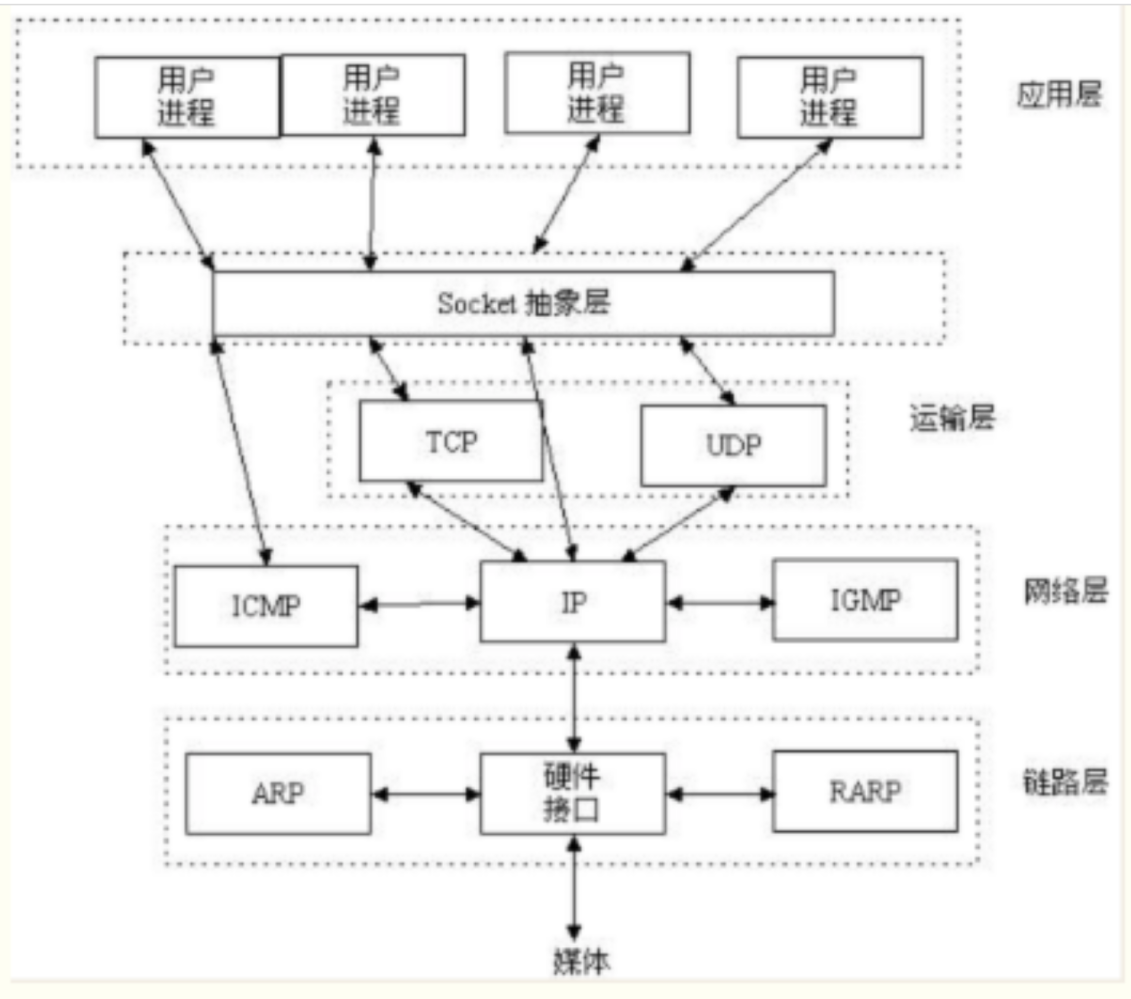
\includegraphics[width=0.8\textwidth]{img/1.png}
    \caption{Socket的地位}
\end{figure}

从某种意义上说,Socket 由地址IP和端口Port构成。IP 是用来标识互联网中的一台主机的位置,而 Port 是用来标识这台机器上的一个应用程序,IP 地址是配置到网卡上的,而 Port 是应用程序开启的,IP 与 Port 的绑定就标识了互联网中独一无二的一个应用程序。

套接字类型 流式套接字(SOCK\_STREAM):用于提供面向连接、可靠的数据传输服务。 数据报套接字(SOCK\_DGRAM):提供了一种无连接的服务。该服务并不能保证数据传输的可靠性,数据有可能在传输过程中丢失或出现数据重复,且无法保证顺序地接收到数据。 原始套接字(SOCK\_RAW):主要用于实现自定义协议或底层网络协议。

在本 WEB 服务器程序实验中,采用流式套接字进行通信。其基本模型如下图所示:
\begin{figure}[htbp]
    \centering
    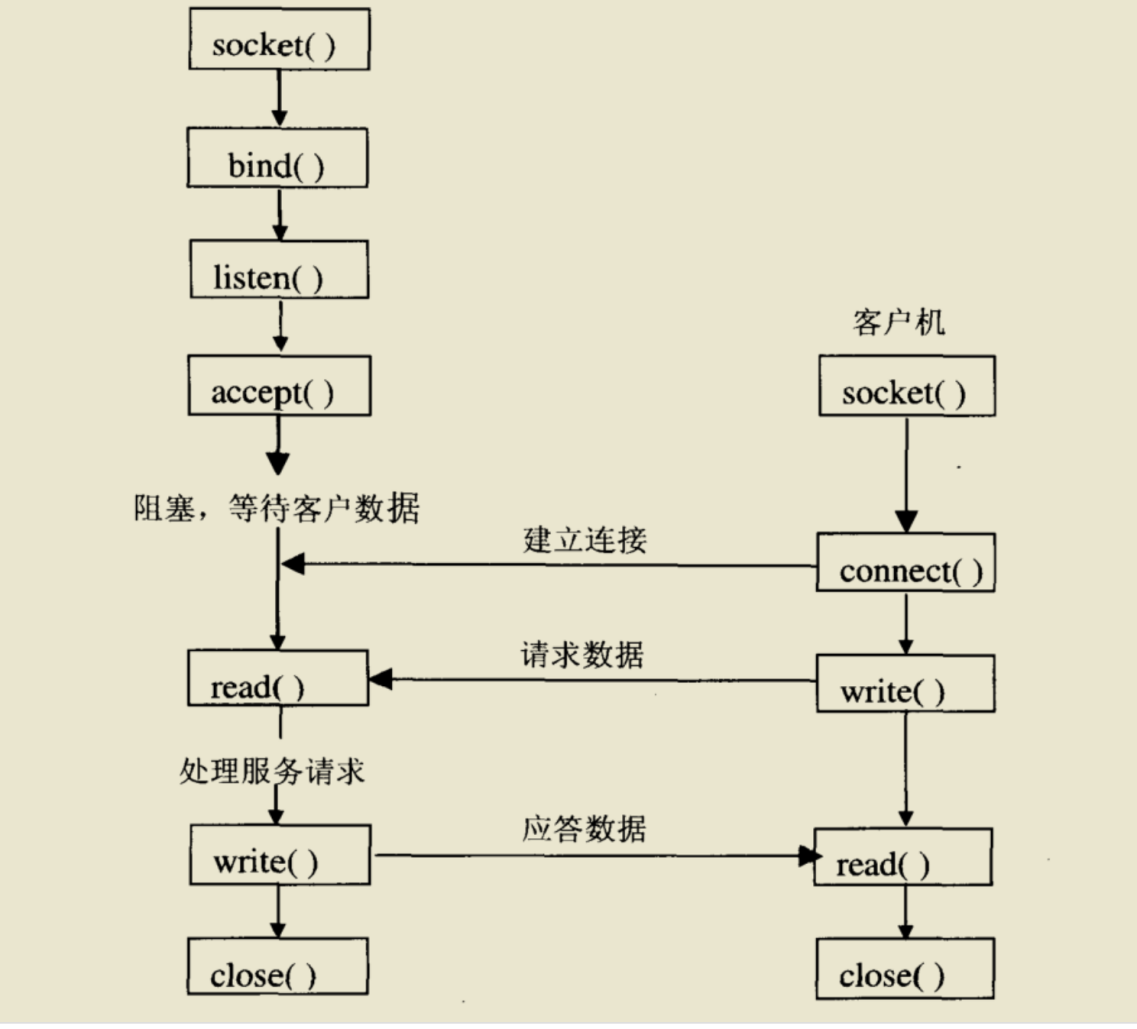
\includegraphics[width=0.8\textwidth]{img/2.png}
    \caption{Socket的基本模型}
\end{figure}

其工作过程如下:服务器首先启动,通过调用 socket()建立一个套接字,然后调用绑定方法 bind()将该套接字和本地网络地址联系在一起,再调用 listen()使套接字做好侦听连接的准备,并设定的连接队列的长度。客户端在建立套接字后,就可调用连接方法 connect()向服务器端提出连接请求。服务器端在监听到连接请求后,建立和该客户端的连接,并放入连接队列中,并通过调用 accept()来返回该连接,以便后面通信使用。客户端和服务器连接一旦建立,就可以通过调用接收方法 recv()/recvfrom()和发送 方法send()/sendto()来发送和接收数据。最后,待数据传送结束后,双方调用 close()关闭套接字。

\subsubsection{HTTP传输协议}
超文本传输协议(HTTP)是用于Web上进行通信的协议:它定义Web浏览器如何从Web服务器请求资源以及服务器如何响应。为简单起见,在该实验中将处理HTTP协议的1.0版。HTTP通信以事务形式进行,其中事务由客户端向服务器发送请求,然后读取响应组成。 请求和响应消息共享一个通用的基本格式:

\begin{itemize}
    \item 初始行(请求或响应行)
    \item 零个或多个头部行
    \item 空行(CRLF)
    \item 可选消息正文
\end{itemize}

对于大多数常见的HTTP事务,协议归结为一系列相对简单的步骤:

首先,客户端创建到服务器的连接;然后客户端通过向服务器发送一行文本来发出请求。这请求行包HTTP方法(比如GET,POST、PUT等),请求URI(类似于URL),以及客户机希望使用的协议版本(比如HTTP/1.0);接着,服务器发送响应消息,其初始行由状态线(指示请求是否成功),响应状态码(指示请求是否成功完成的数值),以及推理短语(一种提供状态代码描述的英文消息组成);最后一旦服务器将响应返回给客户端,它就会关闭连接。

\subsection{实验内容}
建立一个简单的Web服务器端,它能够接收客户端的请求,解析请求的方法和路径,然后返回相应的文件内容作为响应。
\section{实验具体设计实现及结果}
\subsection{实验具体设计实现}
\subsubsection{导入socket模块}
\subsubsection{handle\_request函数}
handle\_request函数用于处理客户端的请求,其主要功能是根据客户端的请求,返回相应的响应报文。

首先,从客户端接收请求报文,接收最多1024个字节的数据,解码成字符串,存储在变量request\_data中;

然后,将请求报文按照回车换行符分割成请求行和请求头部,请求行中包含请求方法、请求资源路径和HTTP版本号,请求头部中包含请求的其他信息;

从第一行中获取请求方法、请求路径和协议版本,如果请求方法是GET则:

如果请求路径是/,则将请求路径设置为/index.html,即默认返回index.html文件;

否则构造文件路径,将请求路径前面的/去掉,尝试打开文件,如果文件不存在,则返回404错误;如果文件存在,则读取文件内容,构造响应报文,将响应头部和响应内容拼接起来,构成完整的响应报文;

如果请求方法不是GET,则返回405错误;

发送响应报文给客户端,关闭连接。

以下是实现代码:

\begin{lstlisting}[title=handle\_request函数,frame=shadowbox]
    def handle_request(client_socket):
    # 接收客户端请求数据从客户端套接字接收最多 1024 字节的数据,并将其解码为字符串,存储在变量 request_data 中,
    request_data = client_socket.recv(1024).decode()

    # 解析请求数据,获取请求文件路径对这个字符串进行分割操作,将其按照回车换行符(\r\n)进行切割,将其拆分成多行。
    request_lines = request_data.split('\r\n')
    if len(request_lines) > 0:
        # 获取请求方法和文件路径
        # method:表示请求方法,如 GET、POST、PUT 等。它是请求行中的第一个部分。
        # path:表示请求的路径,即请求访问的资源在服务器上的位置。它是请求行中的第二个部分。
        method, path, _ = request_lines[0].split(' ')
        if method == 'GET':
            if path == '/':
                # 默认返回 index.html 文件
                file_path = 'index.html'
            else:
                # 构造文件路径
                file_path = path[1:]  # 去除路径中的斜杠

            try:
                # 读取文件内容
                with open(file_path, 'rb') as file:
                    file_content = file.read()
                # 构造响应报文将响应头和文件内容拼接起来,构成完整的响应数据。
                # response_data 变量通过将 response_headers 编码为字节流,并与 file_content 拼接在一起,得到最终的响应数据。
                response_headers = 'HTTP/1.1 200 OK\r\n\r\n'
                response_data = response_headers.encode() + file_content
            except FileNotFoundError:
                # 请求的文件不存在,返回 404 Not Found 错误
                response_headers = 'HTTP/1.1 404 Not Found\r\n\r\n'
                response_data = response_headers.encode()

            # 发送响应数据给客户端
            client_socket.sendall(response_data)
        else:
            response_headers = 'HTTP/1.1 405 Method Not Allowed\r\n\r\n'
            response_data = response_headers.encode()
            client_socket.sendall(response_data)

    # 关闭客户端连接
    client_socket.close()
\end{lstlisting}

\subsubsection{run\_server函数}
run\_server函数用于启动服务器,创建套接字,绑定地址和端口,监听客户端连接,接收客户端请求,处理客户端请求等。

在run\_server函数中:
\begin{itemize}
    \item 创建服务器套接字
    \item 调用bind方法绑定服务器的主机地址和端口号
    \item 调用listen方法开始监听客户端的连接请求。
    \item 进入一个无限循环,等待客户端连接。
    \item 当有客户端连接时,接受连接并获取客户端套接字对象和客户端地址。
    \item 打印客户端连接信息。
\end{itemize}

以下是实现代码:

\begin{lstlisting}[title=run\_server函数,frame=shadowbox]
def run_server():
    # 创建服务器套接字.
    # socket.AF_INET 参数表示使用 IPv4 地址族,socket.SOCK_STREAM 参数表示使用 TCP 协议。
    server_socket = socket.socket(socket.AF_INET, socket.SOCK_STREAM)

    # 调用 server_socket.bind(('localhost', 80)) 绑定服务器的主机地址和端口号。'localhost' 表示服务器在本地主机上运行,80 是服务器的端口号
    server_socket.bind(('localhost', 80))

    # 调用 server_socket.listen(1) 开始监听客户端的连接请求。参数 1 表示允许同时处理的最大连接数为 1。
    server_socket.listen(1)
    print('Server is running on http://localhost:80/')

    while True:
        # 等待客户端连接
        client_socket, addr = server_socket.accept()
        print('Client connected:', addr)
        # 处理客户端请求
        handle_request(client_socket)
\end{lstlisting}

\newpage

\subsection{程序流程图}
\begin{figure}[htbp]
    \centering
    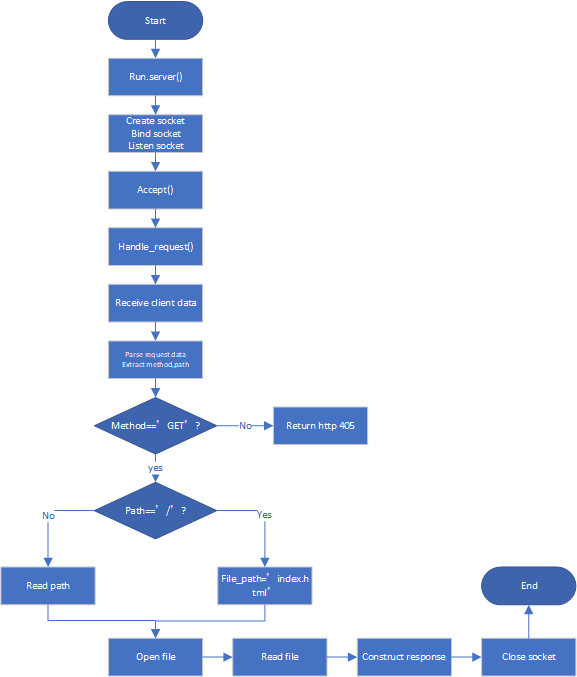
\includegraphics[width=0.8\textwidth]{img/3.png}
    \caption{程序流程图}
\end{figure}

\newpage

\subsection{实验结果}
\subsubsection{启动后控制台输出}
\begin{figure}[htbp]
    \centering
    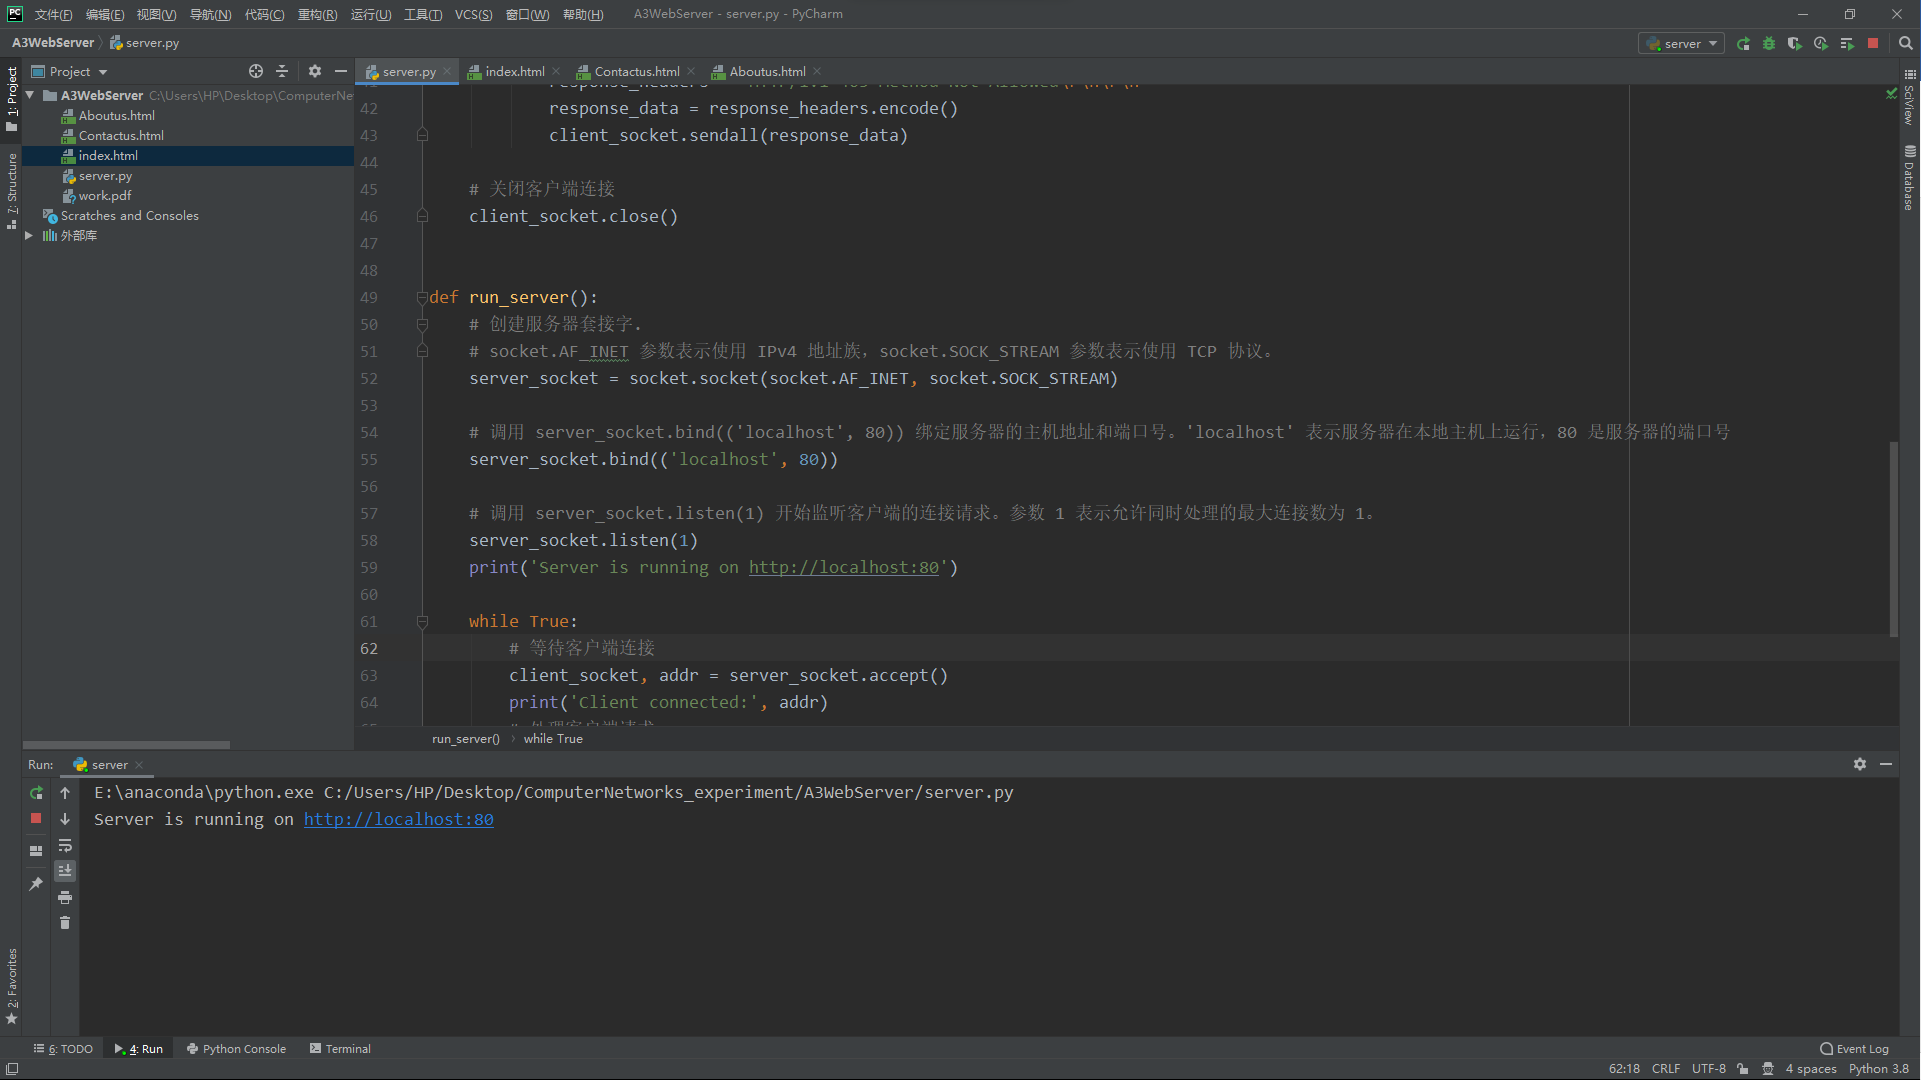
\includegraphics[width=0.7\textwidth]{img/4.png}
    \caption{启动后控制台输出}
\end{figure}

\subsubsection{浏览器默认访问结果}
\begin{figure}[htbp]
    \centering
    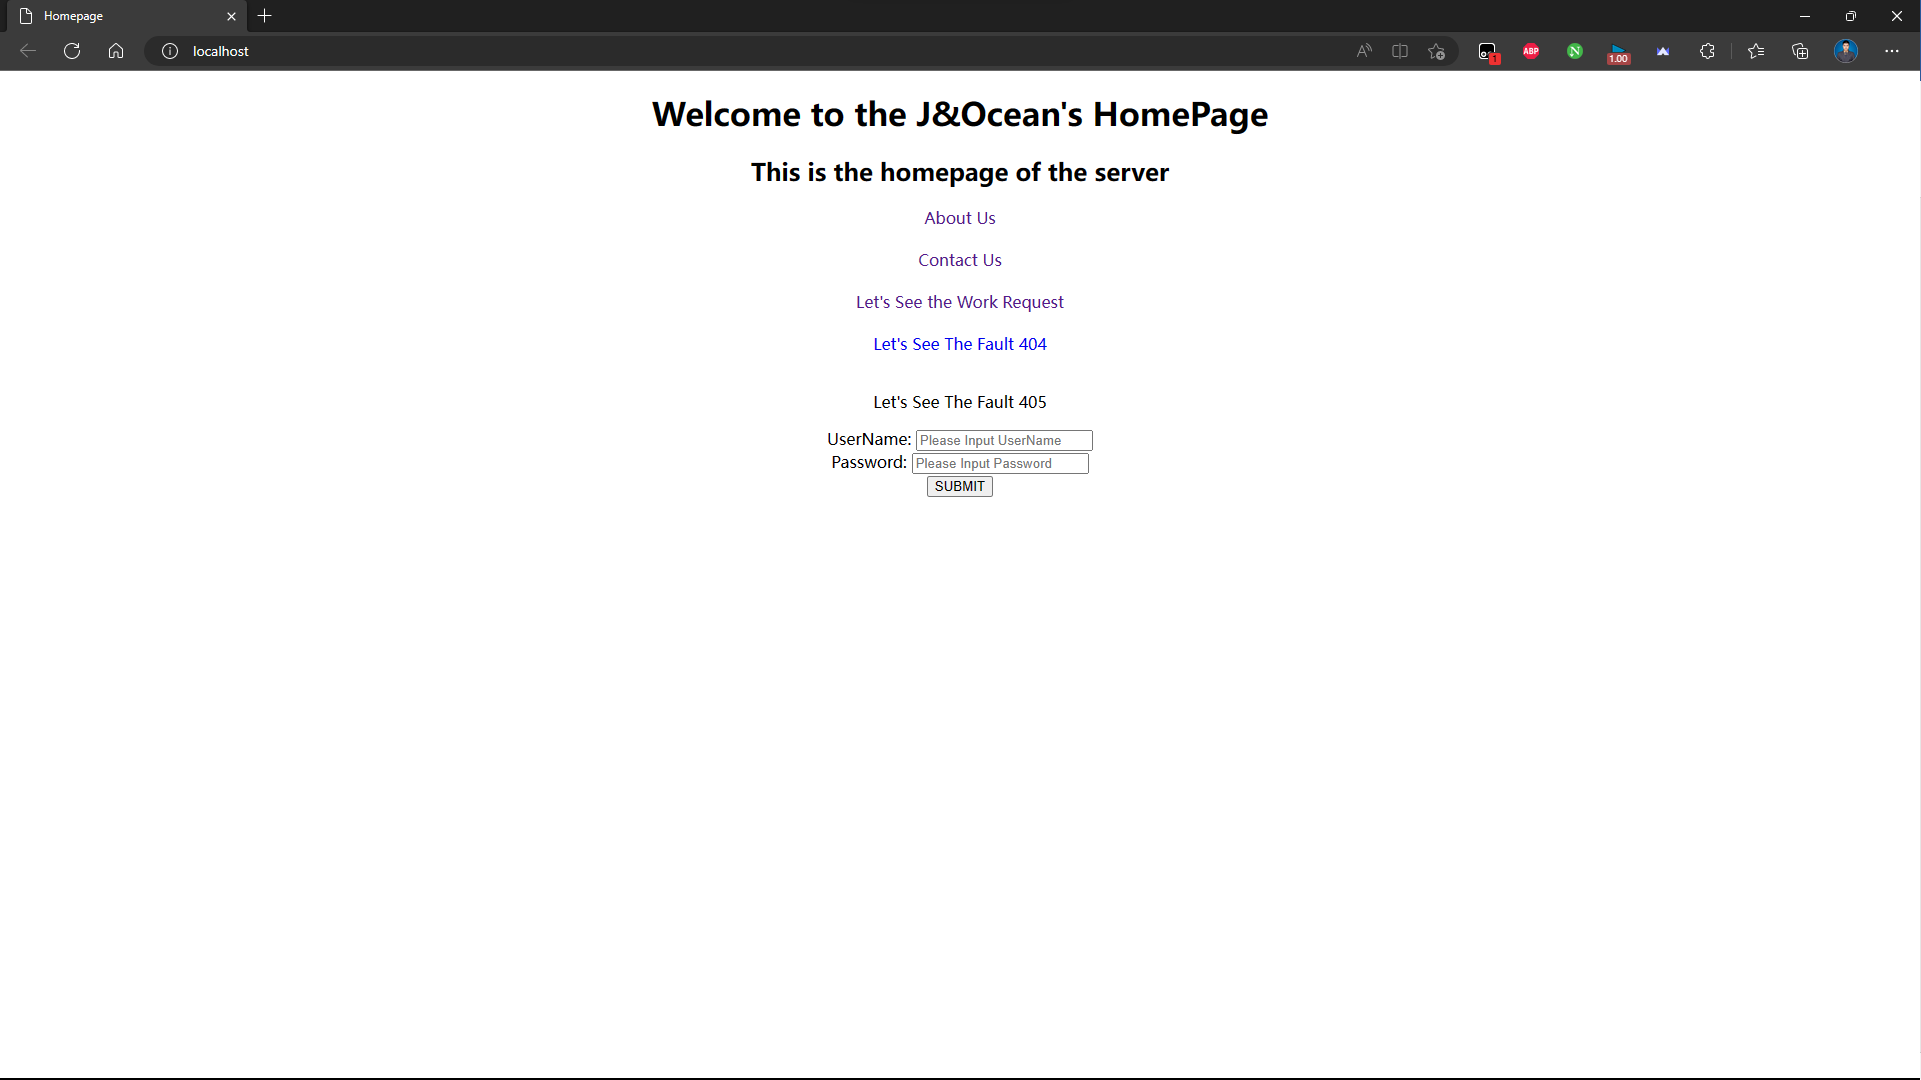
\includegraphics[width=0.7\textwidth]{img/5.png}
    \caption{浏览器默认访问结果}
\end{figure}

\newpage

\subsubsection{浏览器访问Aboutus.html结果}
\begin{figure}[htbp]
    \centering
    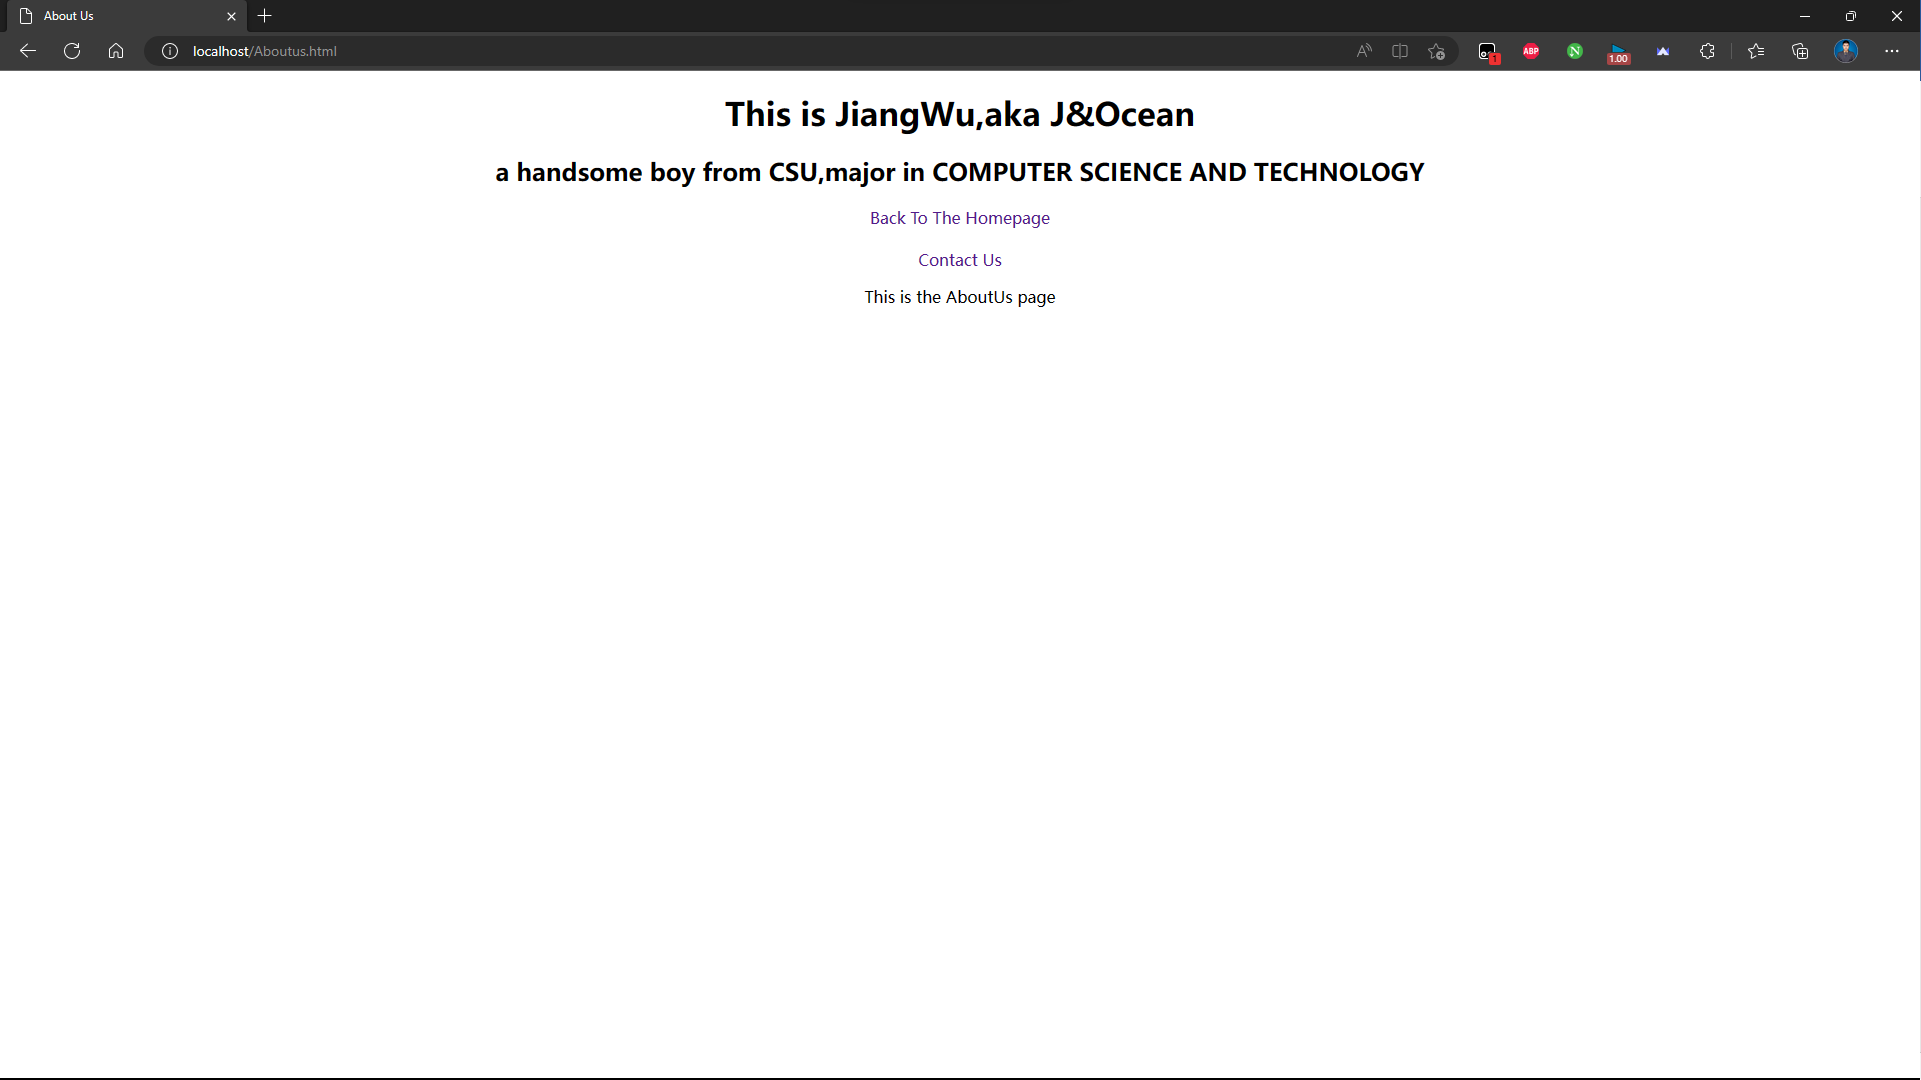
\includegraphics[width=0.7\textwidth]{img/6.png}
    \caption{浏览器访问Aboutus.html结果}
\end{figure}

\subsubsection{浏览器访问Contactus.html结果}
\begin{figure}[htbp]
    \centering
    
\includegraphics[width=0.7\textwidth]{img/7.png}
    \caption{浏览器访问Contactus.html结果}
\end{figure}

\newpage

\subsubsection{浏览器访问work.pdf结果}
\begin{figure}[htbp]
    \centering
    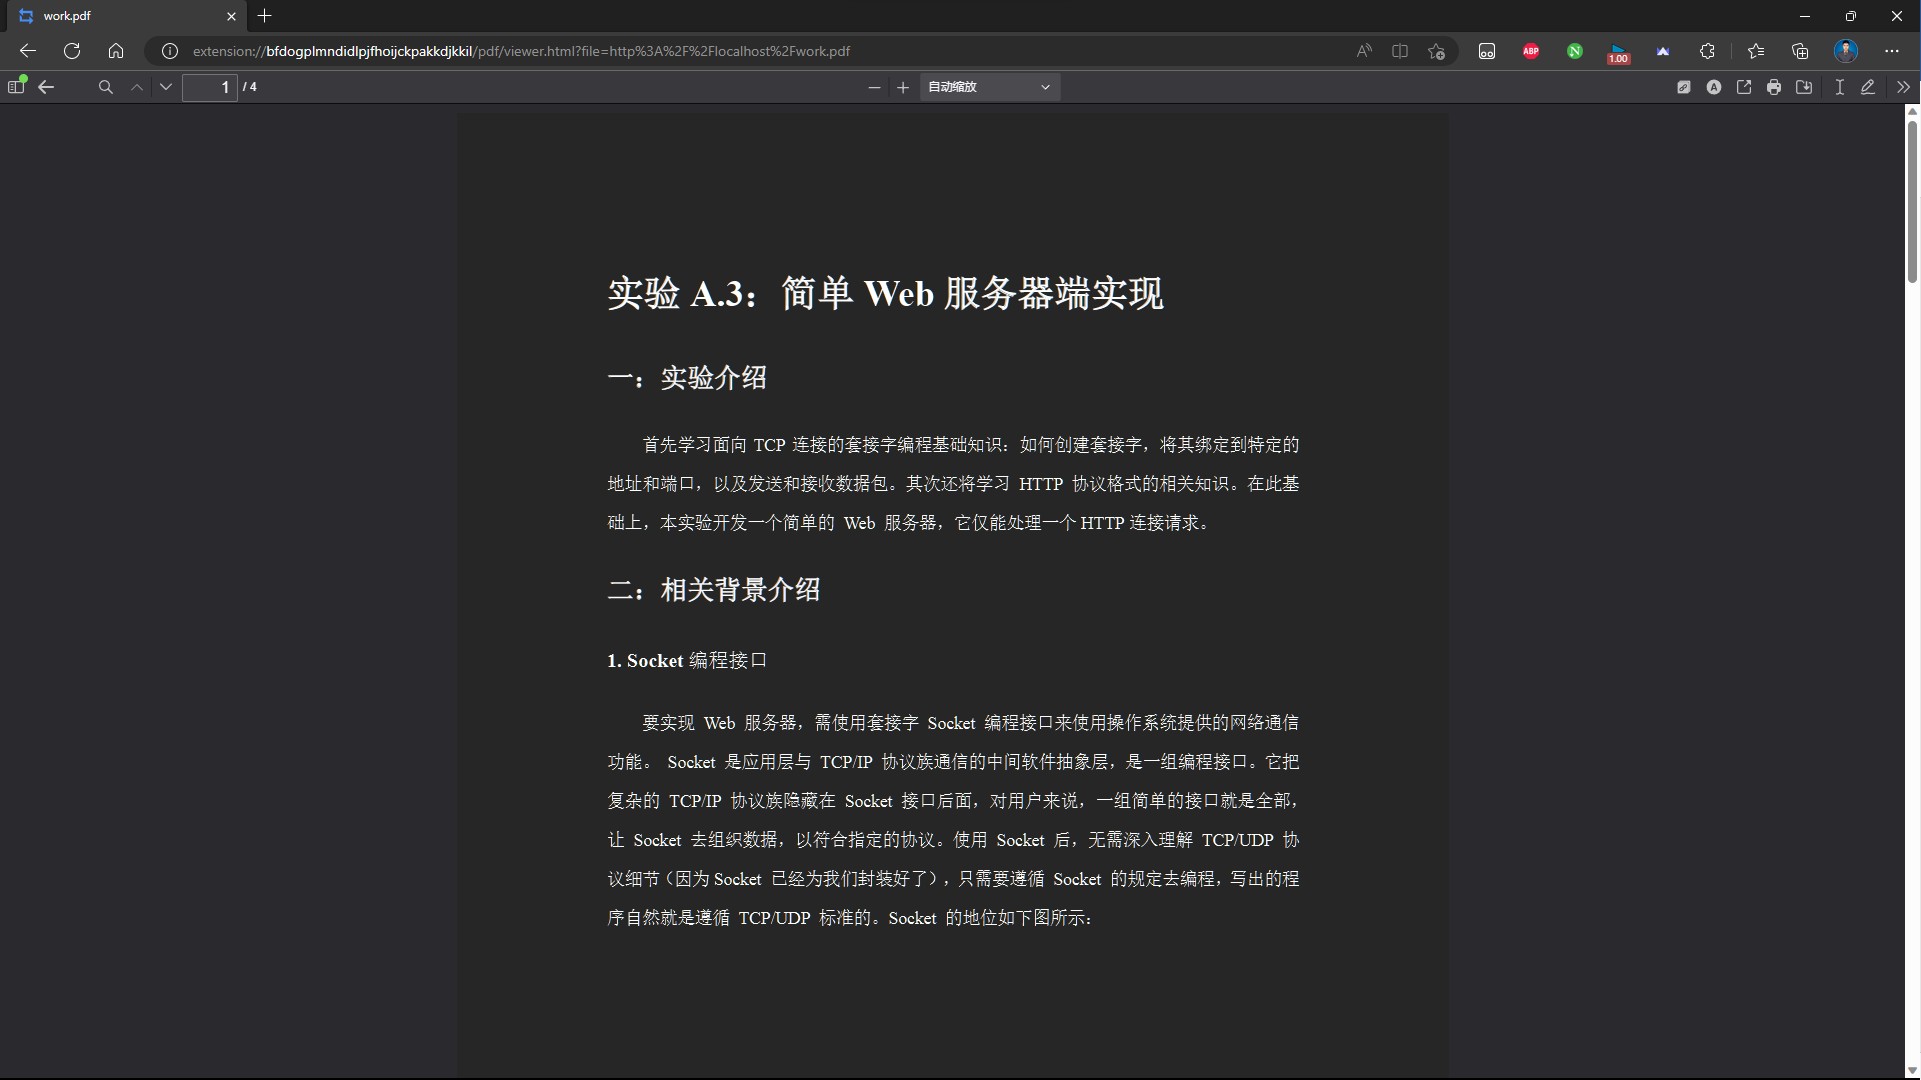
\includegraphics[width=0.7\textwidth]{img/8.png}
    \caption{浏览器访问work.pdf结果}
\end{figure}

\subsubsection{浏览器访问不存在的文件结果}
\begin{figure}[htbp]
    \centering
    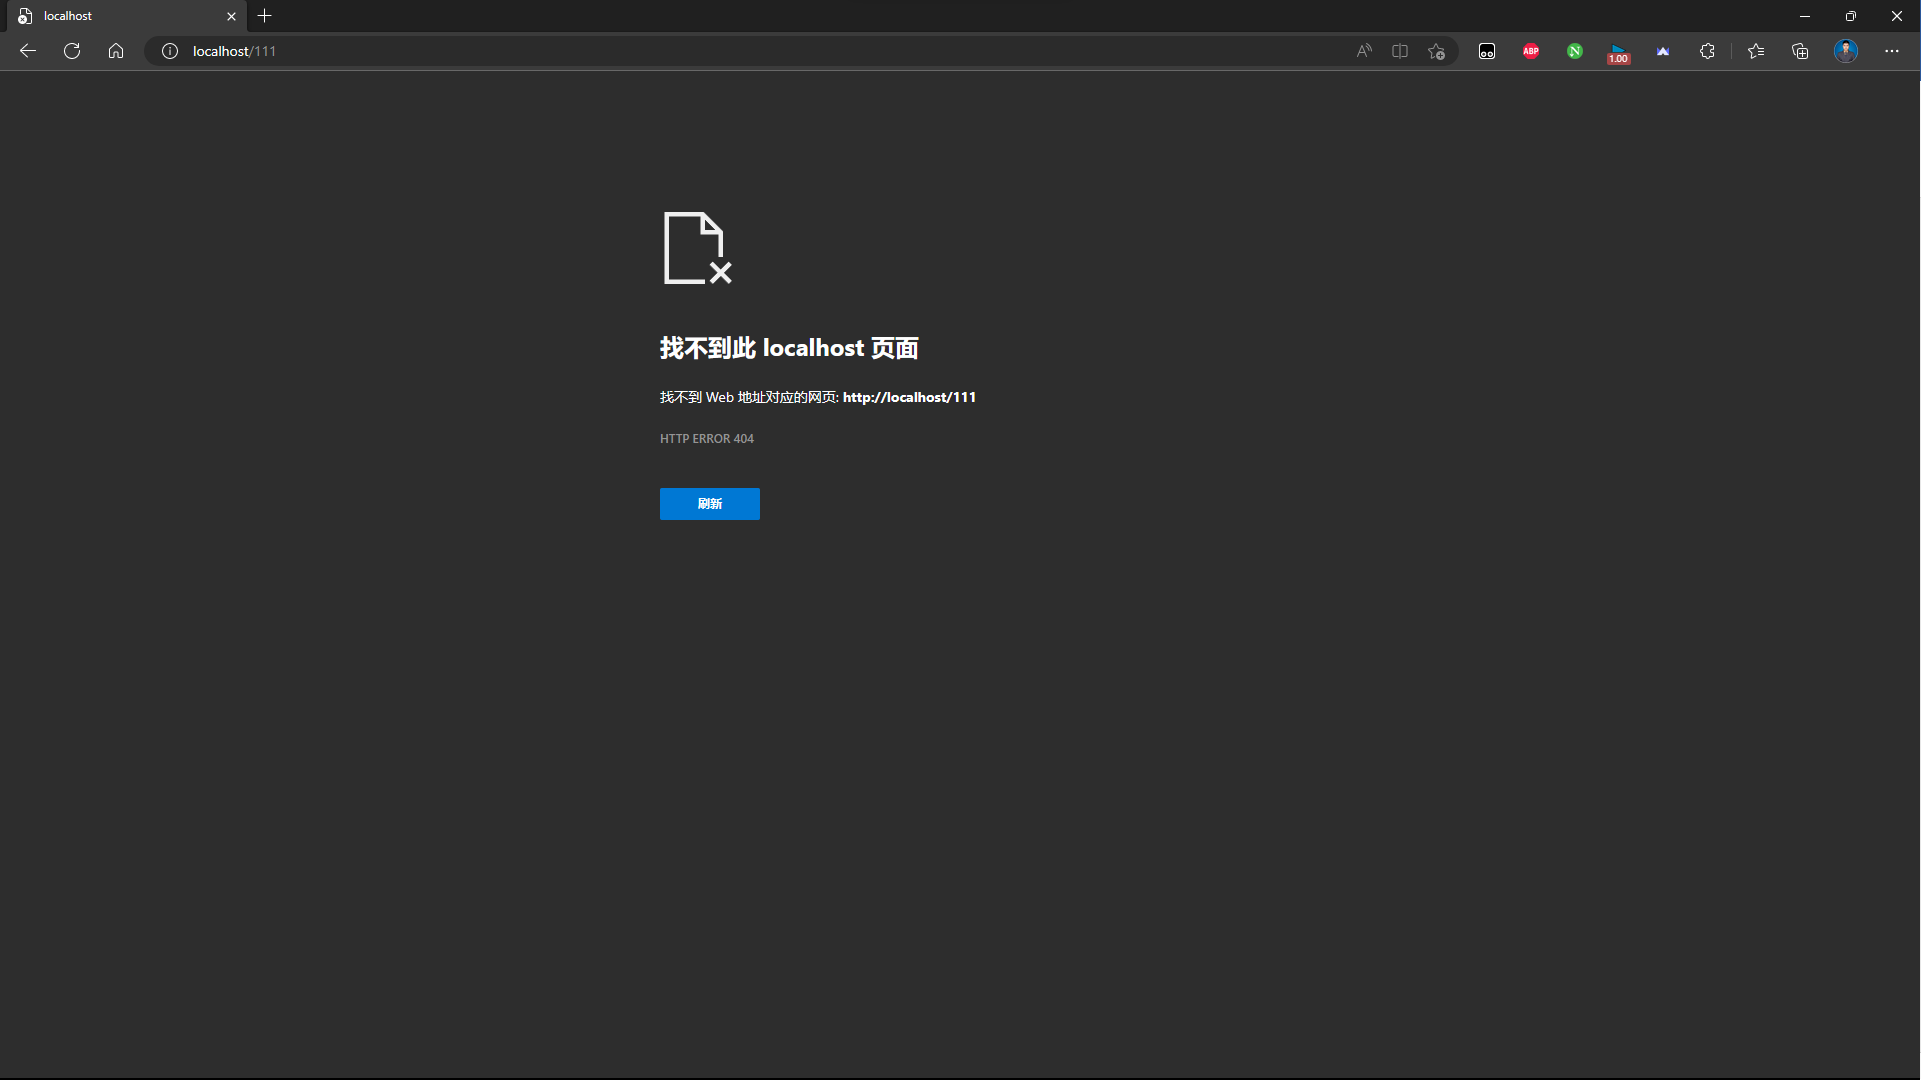
\includegraphics[width=0.7\textwidth]{img/9.png}
    \caption{浏览器访问不存在的文件结果}
\end{figure}

\newpage

\subsubsection{使用错误方法访问结果}
\begin{figure}[htbp]
    \centering
    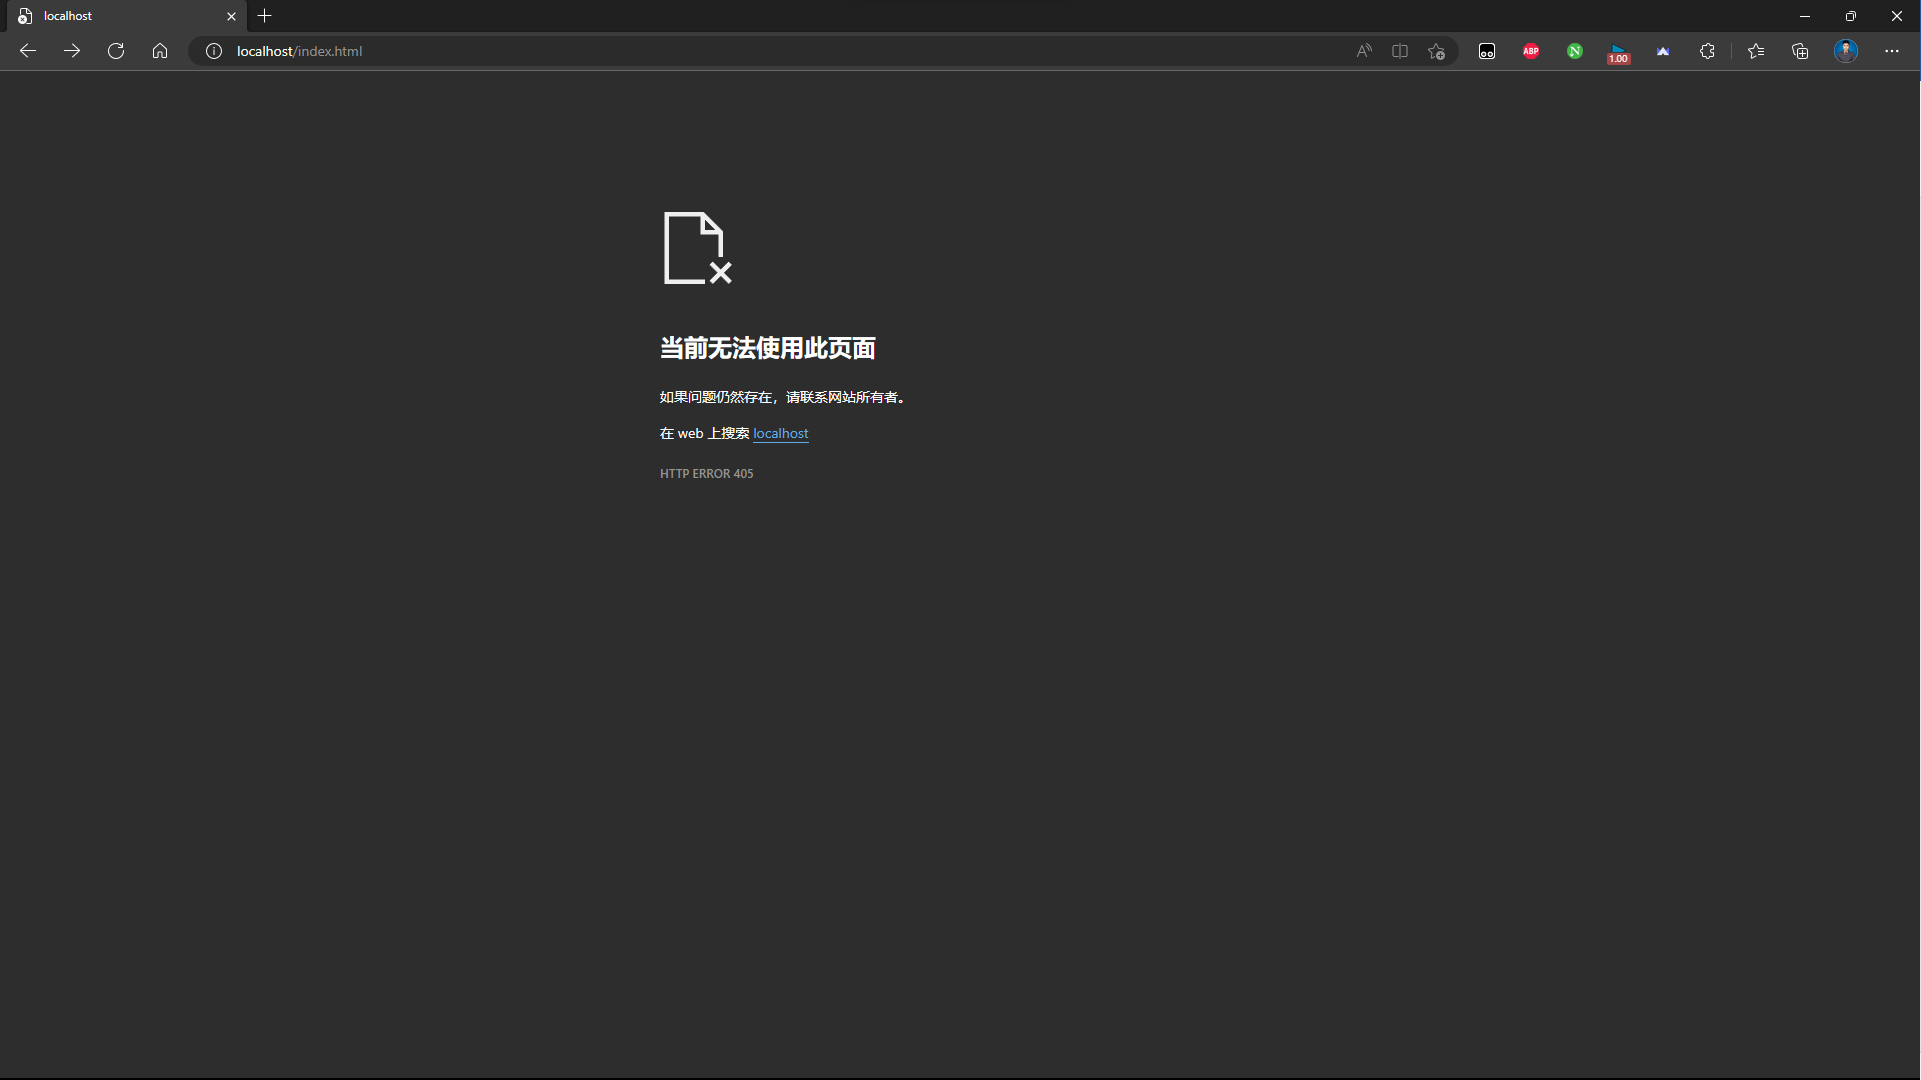
\includegraphics[width=0.7\textwidth]{img/10.png}
    \caption{使用错误方法访问结果}
\end{figure}


\section{实验设备与实验环境}
\begin{enumerate}
    \item 编程语言:python
    \item 编程环境:pycharm,windows11操作系统
\end{enumerate}
\section{实验总结}
在本次实验中,程序实现了一个简单的Web服务器端。该服务器能够接收客户端的请求,解析请求的方法和路径,然后返回相应的文件内容作为响应。
实现过程中遇到的困难:在这个实验中,主要的困难是理解和处理HTTP协议相关的内容。需要熟悉HTTP请求和响应的格式以及常见的状态码。另外,还需要处理文件的读取和异常情况。

通过这个实验,我对基本的Web服务器端实现有了更深入的理解。我学会了使用Python的socket库创建服务器套接字、绑定地址和端口,监听客户端连接请求,并能够处理HTTP请求和构造响应报文。

这个简单的Web服务器端实现还有很大的改进空间。例如,可以添加更多的HTTP方法的支持,如POST、PUT等。还可以引入并发处理多个客户端连接的能力,提高服务器的并发性能。此外,还可以考虑对请求参数进行解析和处理,增加服务器的功能和灵活性。

总体而言,这个实验帮助我更好地理解了Web服务器端的基本原理和实现方式。通过实际编码和调试的过程,我对HTTP协议和socket编程有了更深入的了解,为以后进一步探索网络编程和Web开发打下了坚实的基础。

\section{附录}
\subsection{server.py源码}
\begin{lstlisting}[title=server.py,frame=shadowbox]
    # 实验A.3:简单Web服务器端实现

    import socket
    
    
    def handle_request(client_socket):
        # 接收客户端请求数据从客户端套接字接收最多 1024 字节的数据,并将其解码为字符串,存储在变量 request_data 中,
        request_data = client_socket.recv(1024).decode()
    
        # 解析请求数据,获取请求文件路径对这个字符串进行分割操作,将其按照回车换行符(\r\n)进行切割,将其拆分成多行。
        request_lines = request_data.split('\r\n')
        if len(request_lines) > 0:
            # 获取请求方法和文件路径
            # method:表示请求方法,如 GET、POST、PUT 等。它是请求行中的第一个部分。
            # path:表示请求的路径,即请求访问的资源在服务器上的位置。它是请求行中的第二个部分。
            method, path, _ = request_lines[0].split(' ')
            if method == 'GET':
                if path == '/':
                    # 默认返回 index.html 文件
                    file_path = 'index.html'
                else:
                    # 构造文件路径
                    file_path = path[1:]  # 去除路径中的斜杠
    
                try:
                    # 读取文件内容
                    with open(file_path, 'rb') as file:
                        file_content = file.read()
                    # 构造响应报文将响应头和文件内容拼接起来,构成完整的响应数据。
                    # response_data 变量通过将 response_headers 编码为字节流,并与 file_content 拼接在一起,得到最终的响应数据。
                    response_headers = 'HTTP/1.1 200 OK\r\n\r\n'
                    response_data = response_headers.encode() + file_content
                except FileNotFoundError:
                    # 请求的文件不存在,返回 404 Not Found 错误
                    response_headers = 'HTTP/1.1 404 Not Found\r\n\r\n'
                    response_data = response_headers.encode()
    
                # 发送响应数据给客户端
                client_socket.sendall(response_data)
            else:
                response_headers = 'HTTP/1.1 405 Method Not Allowed\r\n\r\n'
                response_data = response_headers.encode()
                client_socket.sendall(response_data)
    
        # 关闭客户端连接
        client_socket.close()
    
    
    def run_server():
        # 创建服务器套接字.
        # socket.AF_INET 参数表示使用 IPv4 地址族,socket.SOCK_STREAM 参数表示使用 TCP 协议。
        server_socket = socket.socket(socket.AF_INET, socket.SOCK_STREAM)
    
        # 调用 server_socket.bind(('localhost', 80)) 绑定服务器的主机地址和端口号。'localhost' 表示服务器在本地主机上运行,80 是服务器的端口号
        server_socket.bind(('localhost', 80))
    
        # 调用 server_socket.listen(1) 开始监听客户端的连接请求。参数 1 表示允许同时处理的最大连接数为 1。
        server_socket.listen(1)
        print('Server is running on http://localhost:80')
    
        while True:
            # 等待客户端连接
            client_socket, addr = server_socket.accept()
            print('Client connected:', addr)
            # 处理客户端请求
            handle_request(client_socket)
    
    
    run_server()
\end{lstlisting}

\subsection{index.html源码}
\begin{lstlisting}[title=index.html,frame=shadowbox]
    <!DOCTYPE html>
    <html lang="en">
    <head>
        <meta charset="UTF-8">
        <title>Homepage</title>
        <style>
            body{
                text-align: center;
            }
            a{
                text-decoration: none;
            }
            a:hover{
                background: #0000ff;
                color: #fff;
            }
        </style>
    </head>
    <body>
        <h1>Welcome to the J&Ocean's HomePage</h1>
        <h2>This is the homepage of the server</h2>
        <a href="Aboutus.html">About Us</a>
        <br>
        <br>
        <a href="Contactus.html">Contact Us</a>
        <br>
        <br>
        <a href="work.pdf">Let's See the Work Request</a>
        <br>
        <br>
        <a href="111">Let's See The Fault 404</a>
        <br>
        <br>
        <p>Let's See The Fault 405</p>
        <form  method="post">
            <label for="username">UserName:</label>
            <input type="text" name="username" id="username" placeholder="Please Input UserName">
            <br>
            <label for="password">Password:</label>
            <input type="password" name="password" id="password" placeholder="Please Input Password">
            <br>
            <input type="submit" value="SUBMIT">
        </form>
    </body>
    </html>
\end{lstlisting}

\subsection{Aboutus.html源码}
\begin{lstlisting}[title=Aboutus.html,frame=shadowbox]
    <!DOCTYPE html>
    <html lang="en">
    <head>
        <meta charset="UTF-8">
        <title>About Us</title>
        <style>
            body{
                text-align: center;
            }
            a{
                text-decoration: none;
            }
            a:hover{
                background: #0000ff;
                color: #fff;
            }
        </style>
    </head>
    <body>
        <h1>This is JiangWu,aka J&Ocean</h1>
        <h2>a handsome boy from CSU,major in COMPUTER SCIENCE AND TECHNOLOGY</h2>
        <a href="index.html">Back To The Homepage</a>
        <br>
        <br>
        <a href="Contactus.html">Contact Us</a>
        <br>
        <p>This is the AboutUs page</p>
    </body>
    </html>
\end{lstlisting}

\subsection{Contactus.html源码}
\begin{lstlisting}[title=Contactus.html,frame=shadowbox]
    <!DOCTYPE html>
    <html lang="en">
    <head>
        <meta charset="UTF-8">
        <title>Contact Us</title>
        <style>
            body{
                text-align: center;
            }
            a{
                text-decoration: none;
            }
            a:hover{
                background: #0000ff;
                color: #fff;
            }
        </style>
    </head>
    <body>
        <ul>
            <li>QQ:870027163</li>
            <li>GitHub:JIANG-Wu-19</li>
            <li>email:18867576899@163.com</li>
        </ul>
        <a href="index.html">Back To The Homepage</a>
        <br>
        <br>
        <a href="Aboutus.html">About Us</a>
        <br>
        <p>This is the ContactUs page</p>
    </body>
    </html>
\end{lstlisting}
\end{document}